\documentclass[a4paper,10pt]{article}%
\input{commands.tex}%

\author{Peter Bonventre, Lu\'is A. Pereira}%
\title{Genuine equivariant operads}%

\usepackage{showkeys}%

\usepackage{stmaryrd}

\usepackage{geometry}

\usepackage{tikz}%
\tikzset{%
  treenode/.style = {shape=rectangle, rounded corners,%
                     draw, align=center,%
                     top color=white, bottom color=blue!20},%
  root/.style     = {treenode, font=\Large, bottom color=red!30},%
  env/.style      = {treenode, font=\ttfamily\normalsize},%
  dummy/.style    = {circle,draw,inner sep=0pt,minimum size=2mm}%
}%

\usetikzlibrary[decorations.pathreplacing]

\begin{document}	\maketitle%


\abstract{We build new algebraic structures, which we call genuine equivariant operads, which can be thought of as a hybrid between equivariant operads and coefficient systems.
We then prove an Elmendorf type theorem stating that equivariant operads, with their graph model structure, are equivalent to genuine equivariant operads with their projective model structure.

As an application, we build explicit models for the $N_{\infty}$-operads of Blumberg and Hill.
}

\tableofcontents

\section{Introduction}

No content yet.



\section{Planar and tall maps}

\subsection{Planar structures}


Throughout we will work with trees possessing \textit{planar structures} or, more intuitively, trees embedded into the plane.

Our preferred model for trees will be that of broad posets first introduced by Weiss in \cite{We12} and further worked out by the second author in \cite{Pe16b}. We now define planar structures in this context.


\begin{definition}\label{PLANARIZE DEF}
	Let $T \in \Omega$ be a tree. A \textit{planar structure} of $T$ is an extension of the descendancy partial order $\leq_d$ to a total order $\leq_p$ such that: 
	\begin{itemize}
		\item \textit{Planar}: if $e \leq_p f$ and $e \nleq_d f$ then 
		$g \leq_d f$ implies $e \leq_p g$.
	\end{itemize} 
\end{definition}


\begin{example}
An example of a planar structure on a tree $T$ follows, with $\leq_r$ encoded by the number labels.
\begin{equation}\label{PLANAREX EQ}
	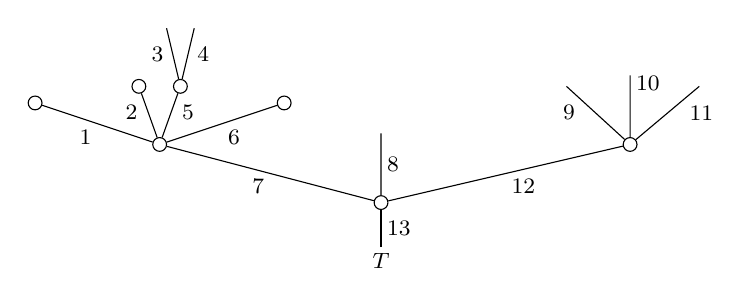
\begin{tikzpicture}[grow=up,auto,level distance=2.1em,
	every node/.style = {font=\footnotesize,inner sep=2pt},
	dummy/.style={circle,draw,inner sep=0pt,minimum size=1.75mm}]
		\node at (0,0) {$T$}
			child{node [dummy] {}
				child[sibling distance = 9em]{node [dummy] {}
					child[sibling distance = 2.5em]{
					edge from parent node [near end,swap] {$11$}}
					child[level distance=2.5em]{
					edge from parent node [very near end,swap] {$10$}}				
					child[sibling distance = 2.3em]{
					edge from parent node [near end] {$9$}}
				edge from parent node [swap] {12}}
				child[level distance =2.5em]{
				edge from parent node [swap] {$8$}}
				child[sibling distance = 8em]{node [dummy] {}
					child[sibling distance =3em, level distance = 1.5 em]{node [dummy] {}
					edge from parent node [swap] {$6$}}
					child[sibling distance = 1.5em]{node [dummy] {}
						child[sibling distance =1em]{
						edge from parent node [swap,near end] {$4$}}
						child[sibling distance =1em]{
						edge from parent node [near end] {$3$}}
					edge from parent node [very near end,swap] {$5$}}
					child[sibling distance =1.5em]{node [dummy] {}
					edge from parent node [very near end] {$2$}}
					child[sibling distance =3em,level distance =1.5em]{node [dummy] {}
					edge from parent node {$1$}}
				edge from parent node {$7$}}
			edge from parent node [swap] {$13$}};
	\end{tikzpicture}
\end{equation}
Intuitively, given a planar depiction of a tree $T$, $e \leq_d f$ holds when the downward path from $e$ passes through $f$
and $e \leq_p f$ holds if either
$e \leq_d f$ or if the downward path from $e$ is to the left of the downward path from $f$ (as measured at the node where the paths intersect).
\end{example}



Intuitively, a planar depiction of a tree amounts to choosing a total order for each of the sets of \textit{input edges} of each node (i.e. those edges immediately above that node).

While we will not need to make this last statement precise, we will nonetheless find it convenient to show that Definition \ref{PLANARIZE DEF} is equivalent to such choosing total orders for each of the sets of input edges.
To do so, we first introduce some notation.


\begin{notation}\label{INPUTPATH NOT}
	Let $T \in \Omega$ be a tree and $e \in T$ and edge. We will denote
	\[ I(e) =\{f \in T \colon e \leq_d f \} \]
and refer to this poset as the \textit{input path of $e$}.
\end{notation}

We will repeatedly use the following, which is a consequence of \cite[Cor. 5.26]{Pe16b}.

\begin{lemma}\label{INCOMPNOTOP}
If $e \leq_d f$, $e \leq_d f'$, then $f,f'$ are $\leq_d$-comparable. 
\end{lemma} 

\begin{proposition}\label{INPUTPATHS PROP}
	Let $T \in \Omega$ be a tree. Then
	\begin{itemize}
		\item[(a)] for any $e \in T$ the finite poset $I(e)$ is totally ordered;
		\item[(b)] the poset $(T,\leq_d)$ has all joins, denoted $\vee$. In fact, $\bigvee_{i} e_i = \min (\bigcap_{i} I(e_i))$.
	\end{itemize}
\end{proposition}

\begin{proof}
	(a) is immediate from Lemma \ref{INCOMPNOTOP}.
To prove (b) we note that 
	$\min (\bigcap_{i} I(e_i))$ exists by (a), and that this is clearly the join $\bigvee{e_i}$.
\end{proof}


\begin{notation}
	Let $T \in \Omega$ be a tree and suppose that $e <_d b$. We will denote by $b^{\uparrow}_e \in T$ the predecessor of $b$ in $I(e)$.
\end{notation}


\begin{proposition}\label{INPUTPREDECESSORPROP PROP}
Suppose $e,f$ are $\leq_d$-incomparable edges of $T$ and write $b= e \vee f$. Then
\begin{itemize}
\item [(a)] $e <_d b$, $f<_d b$ and $b^{\uparrow}_e \neq b^{\uparrow}_f$;
\item [(b)] $b^{\uparrow}_e, b^{\uparrow}_f \in b^{\uparrow}$. In fact $\{b^{\uparrow}_e\} = I(e) \cap b^{\uparrow}$,
$\{b^{\uparrow}_f\} = I(f) \cap b^{\uparrow}$;
\item[(c)] if $e' \leq_d e$, $f' \leq_d f$ then 
$b = e' \vee f'$ and $b^{\uparrow}_{e'} = b^{\uparrow}_{e}$, $b^{\uparrow}_{f'} = b^{\uparrow}_{f}$.
\end{itemize}
\end{proposition}


\begin{proof}
(a) is immediate: the condition $e = g$ (resp. $f = g$) would imply $f \leq_d e$ (resp. $e \leq_d f$)
while the condition $b^{\uparrow}_e = b^{\uparrow}_f$ would provide a predecessor of $b$ in $I(e) \cap I(f)$. 

For (b), note that any relation $a <_d b$ factors as 
$a \leq_d b^{\star}_a <_d b$ for some unique $b^{\**}_a \in b^{\uparrow}$, where uniqueness follows from Lemma \ref{INCOMPNOTOP}. Choosing $a=e$ implies $I(e) \cap b^{\uparrow} = \{b^{\**}_e\}$ and letting $a$ range over edges such that $e \leq_d a <_d b$ shows that $b^{\**}_e$ is in fact the predecessor of $b$.

To prove (c) one reduces to the case $e'=e$, in which case it suffices to check $I(e) \cap I(f') = I(e) \cap I(f)$. But if it were otherwise there would exist an edge $a$ satisfying
$f' \leq_d a <_d f$ and $e \leq_d a$, and this would imply $e \leq_d f$, contradicting our hypothesis.
\end{proof}



\begin{proposition}
\label{TERNARYJOIN PROP}
Let $c = e_1 \vee e_2 \vee e_3$.
Then $c = e_i \vee e_j$ iff $c^{\uparrow}_{e_i} \neq c^{\uparrow}_{e_j}$.

Therefore, all ternary joins in $(T,\leq_d)$ are binary, i.e.
\begin{equation}\label{TERNJOIN EQ}
	c = e_1 \vee e_2 \vee e_3 = e_i \vee e_j
\end{equation}
for some $1\leq i <j \leq 3$, and
(\ref{TERNJOIN EQ}) fails for 
 at most one choice of $1\leq i <j \leq 3$.
\end{proposition}


\begin{proof}
If $c^{\uparrow}_{e_i} \neq c^{\uparrow}_{e_j}$ then
$c = \min\left(I(e_i) \cap I(e_j)\right) = e_i \vee e_j$, whereas the converse follows from Proposition \ref{INPUTPREDECESSORPROP PROP}(a).

The ``therefore'' part follows by noting that 
$c^{\uparrow}_{e_1}$, $c^{\uparrow}_{e_2}$, $c^{\uparrow}_{e_3}$
can not all coincide, or else $c$ would not be the minimum of
$I(e_1) \cap I(e_2) \cap I(e_3)$. 
\end{proof}


\begin{example} In the following example $b = e \vee f$, $c = e \vee f \vee g$, $c^{\uparrow}_e= c^{\uparrow}_f =b$.
\[
	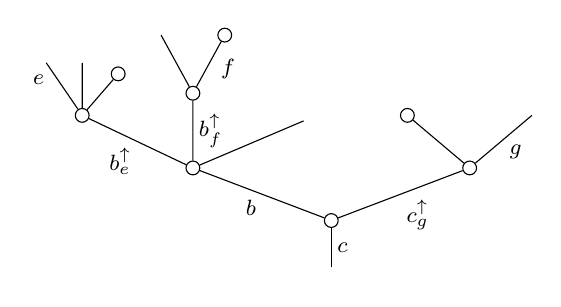
\begin{tikzpicture}[grow=up,auto,level distance=1.9em,
	every node/.style = {font=\footnotesize,inner sep=2pt},
	dummy/.style={circle,draw,inner sep=0pt,minimum size=1.75mm}]
		\node at (0,0) {}
			child{node [dummy] {}
				child[sibling distance = 10em]{node [dummy] {}
					child[sibling distance = 4.5em]{
					edge from parent node [swap] {$g$}}
					child[sibling distance = 4.5em]{node [dummy] {}}
				edge from parent node [swap] {$c_g^{\uparrow}$}}
				child[sibling distance = 10em]{node [dummy] {}
					child[sibling distance = 4em,level distance=1.7em]
					child[sibling distance = 1.5em,level distance=2.7em]{node [dummy] {}
						child[level distance=2.1em,sibling distance = 2.3em]{node [dummy] {}
						edge from parent node [near end,swap] {$f$}}		
						child[level distance=2.1em,sibling distance = 2.3em]{
						edge from parent node [near end] {}}
					edge from parent node [swap] {$b^{\uparrow}_{f}$}}
					child[sibling distance = 4em]{node [dummy] {}
						child[sibling distance =1.3em, level distance = 1.5 em]{node [dummy]  {}
						edge from parent node [swap] {}}
						child[sibling distance = 1.3em]{
						edge from parent node [very near end,swap] {}}
						child[sibling distance =1.3em]{
						edge from parent node [very near end] {$e$}}
					edge from parent node {$b^{\uparrow}_e$}}
				edge from parent node {$b$}}
			edge from parent node [swap] {$c$}};
	\end{tikzpicture}
\]
\end{example}

\begin{notation}
	Given a set $S$ of size $n$ we write
	$\textsf{Ord}(S) \simeq \mathsf{Iso}(S,\{1,\cdots,n\})$. We will usually abuse notation by regarding its objects as pairs $(S,\leq)$ where $\leq$ is a total order in $S$.
\end{notation}


\begin{proposition}\label{PLANARIZATIONCHAR PROP}
	Let $T \in \Omega$ be a tree. There is a bijection
	\begin{equation}\label{PLANAR EQ}
	\begin{tikzcd}[row sep = 0.5em]
		\{\text{planar structures }(T,\leq_p)\} \ar[r] &
		\prod_{(a^{\uparrow} \leq a) \in V(T)} \mathsf{Ord}(a^{\uparrow}) \\
		\leq_p \ar[mapsto]{r} & (\leq_p|_{a^{\uparrow}})
	\end{tikzcd}	
	\end{equation}
\end{proposition}


\begin{proof}
We will keep the setup of Proposition \ref{INPUTPREDECESSORPROP PROP} throughout: $e, f$ are $\leq_d$-incomparable edges and we write $b = e \vee f$. 

	We first show that (\ref{PLANAR EQ}) is injective, i.e. that the restrictions $\leq_p|_{a^{\uparrow}}$ determine if 
	$e <_p f$ holds or not.
If $b^{\uparrow}_e <_p b^{\uparrow}_f$, the relations
$e \leq_d b^{\uparrow}_e <_p b^{\uparrow}_f \geq_d f$
and Definition \ref{PLANARIZE DEF} imply it must be $e <_p f$.
Dually, if $b^{\uparrow}_f <_p b^{\uparrow}_e$ then 
$f <_p e$. Thus 
$b^{\uparrow}_e <_p b^{\uparrow}_f \Leftrightarrow e <_p f$ and hence (\ref{PLANAR EQ}) is indeed injective.

To check that (\ref{PLANAR EQ}) is surjective, it suffices (recall that $e,f$ are assumed $\leq_d$-incomparable) to check that
defining $e \leq_p f$ to hold iff $b^{\uparrow}_e < b^{\uparrow}_f$ holds in $b^{\uparrow}$ yields a planar structure.

Antisymmetry and the total order conditions are immediate, and it thus remains to check the transitivity and planar conditions.
Transitivity of $\leq_p$ in the case $e' \leq_d e <_p f$ and the planar condition, which is the case $e <_p f \geq_d f'$, follow from Proposition \ref{INPUTPREDECESSORPROP PROP}(c). Transitivity of $\leq_p$ in the case $e <_p f \leq_d f'$
follows since either $e \leq_d f'$ or else $e,f'$ are $\leq_d$-incomparable, in which case one can apply \ref{INPUTPREDECESSORPROP PROP}(c) with the roles of $f,f'$ reversed.

It remains to check transitivity in the hardest case, that of 
$e <_p f <_p g$ with $\leq_d$-incomparable $f,g$.
We write $c = e \vee f \vee g$.
By the ``therefore'' part of Proposition \ref{TERNARYJOIN PROP}, either
\begin{inparaenum}
	\item[(i)] $e \vee f <_d c$, in which case 
	Proposition \ref{TERNARYJOIN PROP}
	implies 
	$c^{\uparrow}_e = c^{\uparrow}_f$ and transitivity follows;
	\item[(ii)] $f \vee g <_d c$, which follows just as (i);
	\item[(iii)]  
$e \vee f = f \vee g =c$, in which case 
$c^{\uparrow}_e <
c^{\uparrow}_f <
c^{\uparrow}_g $ in $c^{\uparrow}$
so that $c^{\uparrow}_e \neq c^{\uparrow}_g$ and by Proposition \ref{TERNARYJOIN PROP} it is also 
$e \vee g = c$ and transitivity follows.
\end{inparaenum}
\end{proof}


\begin{remark}\label{FORESTPLAN REM}
	Definition \ref{PLANARIZE DEF} readily extends to forests $F \in \Phi$. The analogue of Proposition \ref{PLANARIZATIONCHAR PROP} then states that the data of a planar structure is 
equivalent to total orderings of the nodes of $F$ together with a total ordering of its set of roots.
Indeed, this follows by either adapting the proof above or by noting that planar structures on $F$ are clearly in bijection with planar structures on the join tree $F \star \eta$ 
(cf. \cite[Def. 7.44]{Pe16b}), which adds a single edge $\eta$ to $F$, serving as the (unique) root of $F \star \eta$.
\end{remark}


When discussing the substitution procedure in \S \ref{SUBS SEC} we will find it convenient to work with a model for the category $\Omega$ that possesses exactly one representative of each possible planar structure on each tree or, more precisely, such that the only isomorphisms preserving the planar structures are the identities. On the other hand, using such a model for $\Omega$ throughout would, among other issues, make the discussion of faces in \S \ref{OUTTALL SEC} rather awkward.
We now outline our conventions to address such issues.


Let $\Omega^p$, the category of \textit{planarized trees}, denote the category with objects pairs $T_{\leq_p}=(T,\leq_p)$ of trees together with a planar structure  and morphisms the \textit{underlying} maps of trees (so that the planar structures are ignored).
There is a full subcategory $\Omega^s \hookrightarrow \Omega^p$, whose objects we call \textit{standard models}, of those $T_{\leq_p}$ whose underlying set is one of the sets $\underline{n} = \{1,2,\cdots,n\}$ and for which $\leq_p$ coincides with the canonical order. 
\begin{example}\label{STANDMODEL EX}
	Some examples of standard models, i.e. objects of $\Omega^s$, follow (further, (\ref{PLANAREX EQ}) can also be interpreted as such an example).
\begin{equation}\label{PLANAROMEGAEX1 EQ}
	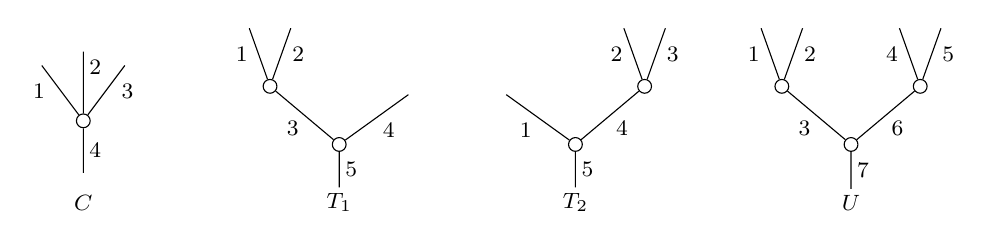
\begin{tikzpicture}[grow=up,auto,level distance=2.1em,
	every node/.style = {font=\footnotesize,inner sep=2pt},
	dummy/.style={circle,draw,inner sep=0pt,minimum size=1.75mm}]
		\node at (-0.25,0) {$C$};
		\node at (-0.25,0.3) {}
			child{node [dummy] {}
				child[sibling distance = 1.5em,level distance= 2em]{
				edge from parent node [swap, near end] {$3$}}
				child[sibling distance = 1.5em,level distance= 2.5em]{
				edge from parent node [swap, near end] {$2$}}
				child[sibling distance = 1.5em,level distance= 2em]{
				edge from parent node [near end] {$1$}}
			edge from parent node [swap] {$4$}};
		\node at (3,0) {$T_1$}
			child{node [dummy] {}
				child[sibling distance = 5em, level distance=1.8em]{
				edge from parent node [swap] {$4$}}
				child[sibling distance = 5em]{node [dummy] {}
					child[sibling distance = 1.5em]{
					edge from parent node [swap,near end] {$2$}}
					child[sibling distance = 1.5em]{
					edge from parent node [near end] {$1$}}
				edge from parent node {$3$}}
			edge from parent node [swap] {$5$}};
		\node at (6,0) {$T_2$}
			child{node [dummy] {}
				child[sibling distance = 5em]{node [dummy] {}
					child[sibling distance = 1.5em]{
					edge from parent node [swap,near end] {$3$}}
					child[sibling distance = 1.5em]{
					edge from parent node [near end] {$2$}}
				edge from parent node [swap] {$4$}}
				child[sibling distance = 5em, level distance=1.8em]{
				edge from parent node {$1$}}
			edge from parent node [swap] {$5$}};
		\node at  (9.5,0) {$U$}
			child{node [dummy] {}
				child[sibling distance = 5em]{node [dummy] {}
					child[sibling distance = 1.5em]{
					edge from parent node [swap,near end] {$5$}}
					child[sibling distance = 1.5em]{
					edge from parent node [near end] {$4$}}
				edge from parent node [swap] {$6$}}
				child[sibling distance = 5em]{node [dummy] {}
					child[sibling distance = 1.5em]{
					edge from parent node [swap,near end] {$2$}}
					child[sibling distance = 1.5em]{
					edge from parent node [near end] {$1$}}
				edge from parent node {$3$}}
			edge from parent node [swap] {$7$}};
	\end{tikzpicture}
\end{equation}
Here $T_1$ and $T_2$ are isomorphic to each other but not isomorphic to any other standard model in $\Omega^s$ while both $C$ and $U$ are the unique objects in their isomorphism classes. 
\end{example}


Given $T_{\leq_p} \in \Omega^p$ there is an obvious standard model $T_{\leq_p}^s \in \Omega^s$ given by replacing each edge by its order following $\leq_p$. Indeed, this defines a retraction 
$(\minus)^s \colon \Omega^p \to \Omega^s$
and a natural transformation 
$\sigma \colon id \Rightarrow (\minus)^s$
given by isomorphisms preserving the planar structure
(in fact, the pair $\left((\minus)^s, \sigma \right)$ is clearly unique).


\begin{convention}\label{PLANARCONV CON}
	From now on, we will write simply $\Omega$, $\Omega_G$ to denote the categories $\Omega^s$, $\Omega_G^s$ of standard models (where planar structures are defined in the underlying forest as in Remark \ref{FORESTPLAN REM}). 
Similarly $\mathsf{O}_G$ will denote the model $\mathsf{O}_G^s$ for the orbital category whose objects are the orbital $G$-sets whose underlying set is one of the sets $\underline{n} = \{1,2,\cdots,n\}$.

Therefore, whenever one of our constructions produces an object/diagram in $\Omega^p$, $\Omega^p_G$, $\mathsf{O}_G^p$ (of trees, $G$-trees, orbital $G$-sets with a planarization/total order) we will hence implicitly reinterpret it by using the standardization functor $(\minus)^s$.
\end{convention}

\begin{example}
To illustrate our convention, we consider the trees in Example \ref{STANDMODEL EX}. 

One has subfaces
$F_1 \subset F_2 \subset U$
where $F_1$ is the subtree with edge set $\{1,2,6,7\}$ and 
$F_2$ is the subtree with edge set $\{1,2,3,6,7\}$, both with inherited tree and planar structures. 
Applying $(\minus)^s$ to the inclusion diagram on the left below then yields a diagram as on the right.
\[
\begin{tikzcd}[row sep = 0.5em,column sep =1.3em]
	F_1 \ar[hookrightarrow]{rr} \ar[hookrightarrow]{rd} & & U & &&
	C \ar{rr} \ar{rd} & & U
\\
	& F_2 \ar[hookrightarrow]{ru} & & &&
	& T_1 \ar{ru}
\end{tikzcd}
\]
Similarly, let $\leq_{(12)}$ and $\leq_{(45)}$ denote alternate planar structures for $U$ exchanging the orders of the pairs $1,2$ and $4,5$, so that one has objects 
$U_{\leq_{(12)}}$, $U_{\leq_{(45)}}$ in $\Omega^p$. 
Applying $(\minus)^s$ to the diagram of underlying identities on the left yields the permutation diagram on the right.
\[
\begin{tikzcd}[row sep = 0.5em,column sep =1.3em]
	U \ar{rr}{id} \ar{rd}[swap]{id} & & U_{\leq_{(45)}} & & &
	U \ar{rr}{(45)} \ar{rd}[swap]{(12)} & & U
\\
	& U_{\leq_{(12)}} \ar{ru}[swap]{id} & & & &
	& U \ar{ru}[swap]{(12)(45)}
\end{tikzcd}
\]
\end{example}

\begin{example}
An additional reason to leave the use of $(\minus)^s$ implicit
is that when depicting $G$-trees it is preferable to choose edge labels that describe the action rather than the planarization (which is already implicit anyway).

For example, when $G = \mathbb{Z}_{/4}$, in both diagrams below the orbital representation on the left represents the isomorphism class consisting of the two trees $T_1,T_2 \in \Omega_G$ on the right.
\[
	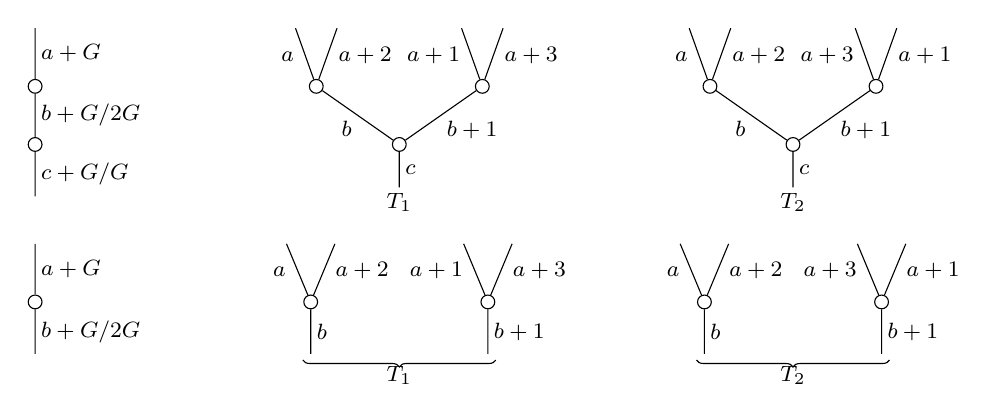
\begin{tikzpicture}[grow=up,auto,level distance=2.1em,
	every node/.style = {font=\footnotesize,inner sep=2pt},
	dummy/.style={circle,draw,inner sep=0pt,minimum size=1.75mm}]
		\node at (-1,0) {}
			child{node [dummy] {}
				child{node [dummy] {}
					child{
					edge from parent node [swap] {$a+G$}}
				edge from parent node [swap] {$b+G/2G$}}
			edge from parent node [swap] {$c + G/G$}};

		\node at  (3.625,0) {$T_1$}
			child{node [dummy] {}
				child[sibling distance = 6em]{node [dummy] {}
					child[sibling distance = 1.5em]{
					edge from parent node [swap,near end] {$a+3$}}
					child[sibling distance = 1.5em]{
					edge from parent node [near end] {$a+1$}}
				edge from parent node [swap] {$b+1$}}
				child[sibling distance = 6em]{node [dummy] {}
					child[sibling distance = 1.5em]{
					edge from parent node [swap,near end] {$a+2$}}
					child[sibling distance = 1.5em]{
					edge from parent node [near end] {$\phantom{0+}a$}}
				edge from parent node {$\phantom{1+}b$}}
			edge from parent node [swap] {$c$}};
		\node at  (8.625,0) {$T_2$}
			child{node [dummy] {}
				child[sibling distance = 6em]{node [dummy] {}
					child[sibling distance = 1.5em]{
					edge from parent node [swap,near end] {$a+1$}}
					child[sibling distance = 1.5em]{
					edge from parent node [near end] {$a+3$}}
				edge from parent node [swap] {$b+1$}}
				child[sibling distance = 6em]{node [dummy] {}
					child[sibling distance = 1.5em]{
					edge from parent node [swap,near end] {$a+2$}}
					child[sibling distance = 1.5em]{
					edge from parent node [near end] {$\phantom{0+}a$}}
				edge from parent node {$\phantom{1+}b$}}
			edge from parent node [swap] {$c$}};
		\node at (-1,-2) {}
			child{node [dummy] {}
				child[sibling distance=1.75em]{
				edge from parent node [swap]  {$a+G$}}
			edge from parent node [swap] {$b+G/2G$}};
		\node at (2.5,-2) {}
			child{node [dummy] {}
				child[sibling distance=1.75em]{
				edge from parent node [swap,near end] {$a+2$}}
				child[sibling distance=1.75em]{
				edge from parent node [near end]  {$\phantom{1+}a$}}
			edge from parent node [swap] {$b$}};
		\node at (4.75,-2) {}
			child{node [dummy] {}
				child[sibling distance=1.75em]{
				edge from parent node [swap,near end] {$a+3$}}
				child[sibling distance=1.75em]{
				edge from parent node [near end]  {$a+1$}}
			edge from parent node [swap] {$b+1$}};
		\draw[decorate,decoration={brace,amplitude=2.5pt}] (4.85,-2) -- (2.4,-2) node[midway]{$T_1$};
		\node at (7.5,-2) {}
			child{node [dummy] {}
				child[sibling distance=1.75em]{
				edge from parent node [swap,near end] {$a+2$}}
				child[sibling distance=1.75em]{
				edge from parent node [near end]  {$\phantom{1+}a$}}
			edge from parent node [swap] {$b$}};
		\node at (9.75,-2) {}
			child{node [dummy] {}
				child[sibling distance=1.75em]{
				edge from parent node [swap,near end] {$a+1$}}
				child[sibling distance=1.75em]{
				edge from parent node [near end]  {$a+3$}}
			edge from parent node [swap] {$b+1$}};
		\draw[decorate,decoration={brace,amplitude=2.5pt}] (9.85,-2) -- (7.4,-2) node[midway]{$T_2$};
	\end{tikzpicture}
\]
\end{example}


\begin{definition}
	A morphism $S \xrightarrow{\varphi} T$ in $\Omega$ that is compatible with the planar structures $\leq_p$ is called a 
	\textit{planar map}.
	
	More generally, a morphism $F \to G$ in the categories $\Phi$, $\Phi^G$, $\Omega^G$ of forests, $G$-forests, $G$-trees is called a \textit{planar map} if it is an independent map (cf. \cite[Def. 5.28]{Pe16b}) compatible with the planar structures $\leq_p$.
\end{definition}


\begin{remark}
	The need for the independence condition is justified by \cite[Lemma 5.33]{Pe16b} and its converse, since non independent maps do not reflect
 $\leq_d$ inequalities.
 
 We note that in the $\Omega_G$ case a map $\varphi$ is independent iff $\varphi$ does not factor through a non trivial quotient iff $\varphi$ is injective on each edge orbit.
\end{remark}


\begin{proposition}
\label{PLANARPULL EQ}
	Let $F \xrightarrow{\varphi} G$ be an independent map in $\Phi$ (or $\Omega$, $\Omega_G$, $\Phi_G$). Then there is a unique factorization 
	\[F \xrightarrow{\simeq} \bar{F} \to G\]
	such that $F \xrightarrow{\simeq} \bar{F}$ is an isomorphism and $\bar{F} \to G$ is planar.
\end{proposition}

\begin{proof}
We need to show that there is a unique planar structure 
$\leq_p^{\bar{F}}$ on the underlying forest of $F$ making the underlying map a planar map.
Simplicity of $G$ ensures that for any vertex $e^{\uparrow} \leq e$ of $F$ the edges in $\varphi(e^{\uparrow})$ are all distinct while independence of $\varphi$ likewise ensures that the edges in $\varphi(\underline{r}_F)$ are distinct.
The result now follows from (the forest version of) Proposition
\ref{PLANARIZATIONCHAR PROP}: one simply orders each set $e^{\uparrow}$ and $\underline{r}_F$ according to its image.

{\color{orange} not quite complete... maybe that $\leq_p$ is the closure of $\leq_d$ and the vertex relations under transitivity and the planar condition}
\end{proof}



\begin{remark}\label{PULLPLANAR REM}
	Proposition \ref{PLANARPULL EQ} says that planar structures  can be pulled back along independent maps. However, they can not always be pushed forward. As an example, in the notation of (\ref{PLANAROMEGAEX1 EQ}), consider the map $C \to T_1$ defined by $1 \mapsto 1$, $2 \mapsto 4$, $3 \mapsto 2$, $4 \mapsto 5$.
\end{remark}

\begin{remark}\label{UNIQCOR REM}
	Given any tree $T \in \Omega$ there is a unique corolla $\mathsf{lr}(T) \in \Sigma$ and planar tall map 
	$\mathsf{lr}(T) \to T$.
	Explicitly, the number of leaves of $\mathsf{lr}(T)$ matches that of $T$, together with the inherited order. 
\end{remark}


\subsection{Outer faces and tall maps}\label{OUTTALL SEC}



In preparation for our discussion of the substitution operation in \S \ref{SUBS SEC}, we now recall some basic notions and results concerning outer subtrees and tree grafting, as in \cite[\S5]{Pe16b}.

\begin{definition}
	Let $T \in \Omega$ be a tree and 
	$e_1 \cdots e_n =\underline{e} \leq e$ a broad relation in $T$.
	
	We define the \textit{planar outer face $T_{\underline{e} \leq e}$}
	to be the subtree with underlying set those edges $f \in T$ such that
\begin{equation}\label{OUTERFACE EQ}
	f \leq_d e,\quad \forall_i e_i \nless_d f,
\end{equation}
generating broad relations the relations $f^{\uparrow} \leq f$ for $f$ satisfying (\ref{OUTERFACE EQ}) and $\forall_i f\neq e_i$,
and planar structure pulled back from $T$.
\end{definition}


\begin{remark}
If one forgoes the requirement that $T_{\underline{e} \leq e}$ be equipped with the pullback planar structure, the inclusion $T_{\underline{e} \leq e} \to T$ is usually called simply an \textit{outer face}.
\end{remark}

We now recap some basic results.

\begin{proposition}
Let $T \in \Omega$ be a tree.
\begin{itemize}
\item[(a)] $T_{\underline{e} \leq e}$ is a tree with root $e$
and edge tuple $\underline{e}$;
\item[(b)] there is a bijection
\[
	\{\text{planar outer faces of $T$} \} 
\leftrightarrow 
	\{\text{broad relations of $T$}\};
\]
\item[(c)] if $R \to S$ and $S \to T$ are outer face maps then so is $R \to T$;
\item[(d)] any pair of broad relations $\underline{g} \leq v$, $\underline{f}v \leq e$ induces a grafting pushout diagram
\begin{equation}\label{GRAPTPUSH EQ}
\begin{tikzcd}
	\eta \ar{r}{v} \ar{d}[swap]{v} & T_{\underline{g} \leq v} \ar{d}
\\
	T_{\underline{f}v \leq e} \ar{r} & T_{\underline{f}\underline{g} \leq v}
\end{tikzcd}
\end{equation}
%\item[(e)] a face map $S \to T$ is an outer face map iff whenever the composite relation $\underline{f} \underline{g} \leq e$ is in $S$ then so are the relations $\underline{g} \leq v$ and
%$\underline{f}v \leq e$.
\end{itemize}
\end{proposition}


\begin{proof}
We first show (a). That $T_{\underline{e} \leq e}$ is indeed a tree is the content of \cite[Prop. 5.20]{Pe16b}: more precisely, 
$T_{\underline{e} \leq e} = (T^{\leq e})_{\less \underline{e}}$
in the notation therein. That the root of $T_{\underline{e} \leq e}$ is $e$ is clear and that the root tuple is $\underline{e}$ follows from \cite[Remark 5.23]{Pe16b}.

 (b) follows from (a), which shows that $\underline{e} \leq e$ can be recovered from
$T_{\underline{e} \leq e}$.

 (c) follows from the definition of outer face together with \cite[Lemma 5.33]{Pe16b}, which states that the $\leq_d$ relations on $S,T$ coincide.
 
  Since by (c) both $T_{\underline{g} \leq v}$ and $T_{\underline{f}v \leq e}$ are outer faces of $T_{\underline{f} \underline{g} \leq v}$, 
(d) is a restatement of \cite[Prop. 5.15]{Pe16b}. 
%Since $\underline{e} \leq e$ is a broad relation in $T_{\underline{e} \leq e}$ (this follows from (a) together with \cite[Lemma 5.13]{Pe16b})
\end{proof}

\begin{definition}
	A map $S \xrightarrow{\varphi} T$ in $\Omega$ is called a \textit{tall map} if 
	\[\varphi(\underline{l}_S) = \underline{l}_T, 
		\qquad
	\varphi(r_S)= r_T,\]
where $l_{(\minus)}$ denotes the leaf tuple and $r_{(\minus)}$ the root.
\end{definition}


The following is a restatement of \cite[Cor. 5.24]{Pe16b}

\begin{proposition}\label{TALLOUTERDEC COR}
	Any map $S \xrightarrow{\varphi} T$ in $\Omega$ has a factorization, unique up to unique isomorphism,
	\[
		S \xrightarrow{\varphi^t} U \xrightarrow{\varphi^u} T
	\]
	as a tall map followed by an outer face (in fact, 
	$U= T_{\varphi(\underline{l}_S) \leq r_S}$).
\end{proposition}

We recall that a face $F \to T$ is called inner if is obtained by iteratively removing inner edges, i.e. edges other than the root or the leaves. In particular, it follows that a face is inner iff it is tall. The usual face-degeneracy decomposition thus combines with Corollary \ref{TALLOUTERDEC COR} to give the following.

\begin{corollary}
	Any map $S \xrightarrow{\varphi} T$ in $\Omega$ has a factorization, unique up to unique isomorphisms,
	\begin{equation}\label{TRIPLEFACT EQ}
		S \xrightarrow{\varphi^-} U \xrightarrow{\varphi^i} V \xrightarrow{\varphi^u} T
	\end{equation}
	as a degeneracy followed by an inner face followed by an outer face.
\end{corollary}
	
\begin{proof}
	The factorization (\ref{TRIPLEFACT EQ}) can be built by first performing the degeneracy-\-face decomposition and then performing the tall-outer decomposition on the face map.
\end{proof}


\subsection{Substitution}\label{SUBS SEC}


One of the key ideas needed to describe operads is that of substitution of tree nodes, a process that we will prefer to repackage in terms of maps of trees. We start by discussing an example, focusing on the related notion of 
 iterated graftings of trees (as described in (\ref{GRAPTPUSH EQ})).

\begin{example} The trees $U_1, U_2,\cdots, U_6$ on the left below can be grafted into the tree $U$ in the middle.
More precisely (among other possible grafting orders), one has
\begin{equation}\label{UFORMULA EQ}
U = \left(
		\left(
			\left(
				\left(
					\left(U_6 \amalg_a U_2 \right)
				\right) \amalg_a U_1
			\right) \amalg_b U_3
		\right) \amalg_d U_5
	\right) \amalg_c U_4
\end{equation}
\begin{equation}\label{SUBSDATUMTREES EQ}
	\begin{tikzpicture}[grow=up,auto,level distance=2.1em,
	every node/.style = {font=\footnotesize,inner sep=2pt},
	dummy/.style={circle,draw,inner sep=0pt,minimum size=1.25mm}]
\begin{scope}[xshift=-2em]
	\begin{scope}
	\tikzstyle{level 2}=[sibling distance=2.25em]%
	\tikzstyle{level 3}=[sibling distance=1.25em]%
		\node at (-0.25,3.2) {$U_1$}
			child{node [dummy] {}
				child
				child{node [dummy] {}
					child
					child
				}
			edge from parent node {$a$}};
	\end{scope}
		\node at (-0.25,1.5) {$U_2$}
			child{
		edge from parent node {$a$}};
		\node at (1.15,1.5) {$U_3$}
			child{node [dummy] {}
		edge from parent node {$b$}};
	\begin{scope}
	\tikzstyle{level 2}=[sibling distance=0.875em]%
		\node at (2.2,3.2) {$U_4$}
			child{node [dummy] {}
				child{node [dummy] {}}
				child{node [dummy] {}}
			edge from parent node {$c$}};
	\end{scope}
	\begin{scope}
		\tikzstyle{level 2}=[sibling distance=1.25em]%
		\node at (2.5,1.5) {$U_5$}
			child{node [dummy] {}
				child{node[dummy] {}}
				child{
				edge from parent node {$c$}}
			edge from parent node [swap] {$d$}};
	\end{scope}
	\begin{scope}
	\tikzstyle{level 2}=[sibling distance=3.5em]%
	\tikzstyle{level 3}=[sibling distance=2.25em]%
		\node at (1,-1) {$U_6$}
			child{node [dummy] {}
				child[sibling distance = 5em]{node [dummy] {}
					child[sibling distance = 3.5em]{edge from parent node [swap,near end] {$d$} }
					child[sibling distance = 3.5em]{edge from parent node [near end] {$b$} }
				}
				child[sibling distance = 7em]{ edge from parent node {$a$} }
			edge from parent node [swap] {$e$}};
	\end{scope}
\end{scope}
\begin{scope}[yshift=1em]
	\begin{scope}[level distance=2.3em]
	\tikzstyle{level 2}=[sibling distance=3.5em]%
	\tikzstyle{level 3}=[sibling distance=2.25em]%
	\tikzstyle{level 4}=[sibling distance=1.25em]%
	\tikzstyle{level 5}=[sibling distance=0.875em]%
		\node at (5.5,0) {$U$}
			child{node [dummy] {}
				child[sibling distance =5em]{node [dummy] {}
					child[sibling distance =3.5em]{node [dummy] {}
						child{node [dummy] {}
						}
						child{node [dummy] {}
							child{node [dummy] {}}
							child{node [dummy] {}}
						edge from parent node [near end] {$c$}}
					edge from parent node [swap, near end] {$d$}}
					child[sibling distance =3.5em]{node [dummy] {}
					edge from parent node [near end] {$b$}}
				}
				child[sibling distance =7em]{node [dummy] {}
					child
					child{node [dummy] {}
						child
						child
					}
				edge from parent node {$a$}}
			edge from parent node [swap] {$e$}};
	\end{scope}
	\begin{scope}[level distance=2.3em]
	\tikzstyle{level 2}=[sibling distance=2.3em]%
	\tikzstyle{level 4}=[sibling distance=1em]%
		\node at (10,0.3) {$T$}
			child{node [dummy] {}
				child{node [dummy] {}
					child{node [dummy] {}
					edge from parent node [swap] {$c$}}	
				edge from parent node [swap] {$d$}}
				child{node [dummy] {}
				edge from parent node [near end,swap] {$b$}}
				child{node [dummy] {}
					child{node [dummy] {}
						child
						child
						child
					edge from parent node {$a_1$}}
				edge from parent node {$a_2$}}
			edge from parent node [swap] {$e$}};
	\end{scope}
	\draw [->,dashed] (8.6,1.25) -- node {$\varphi$} (7.1,1.25);
\end{scope}
	\end{tikzpicture}
\end{equation}
We now consider the tree $T$, which is built by converting each $U_i$ into the corolla $\mathsf{lr}(U_i)$ (cf. Remark \ref{UNIQCOR REM}), and then performing the same grafting operations as in (\ref{UFORMULA EQ}). $T$ can then be regarded as encoding the combinatorics of the iterated grafting in (\ref{UFORMULA EQ}), with alternative ways to reorder operations in (\ref{UFORMULA EQ}) in bijection with ways to assemble $T$ out of its nodes.


One can now therefore think of the iterated grafting (\ref{UFORMULA EQ}) as being instead encoded by the tree $T$ together with the (unique) planar tall maps $\varphi_i$ below.
\begin{equation}\label{SUBSDATUMTREES2 EQ}
	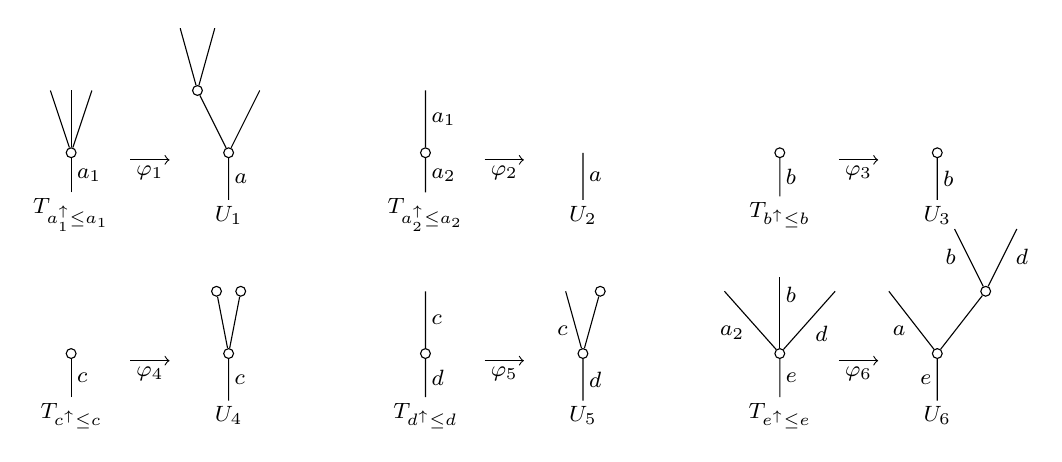
\begin{tikzpicture}[grow=up,auto,level distance=2.25em,
	every node/.style = {font=\footnotesize, inner sep=2pt},
	dummy/.style={circle,draw,inner sep=0pt,minimum size=1.25mm}]
	\begin{scope}
	\tikzstyle{level 2}=[sibling distance=0.75em]%
		\node at (0,0) {$T_{a_1^{\uparrow}\leq a_1}$}
			child{node [dummy] {}
				child
				child
				child
			edge from parent node [swap] {$a_1$}};
	\end{scope}	
	\begin{scope}
	\tikzstyle{level 2}=[sibling distance=2.25em]%
	\tikzstyle{level 3}=[sibling distance=1.25em]%
		\node at (2,0) {$U_1$}
			child{node [dummy] {}
				child
				child{node [dummy] {}
					child
					child
				}
			edge from parent node [swap] {$a$}};
	\end{scope}
		\draw [->] (0.75,0.7) -- node [swap]{$\varphi_1$} (1.25,0.7);
		\node at (4.5,0) {$T_{a_2^{\uparrow}\leq a_2}$}
			child{node [dummy] {}
				child{
				edge from parent node [swap] {$a_1$}}
			edge from parent node [swap] {$a_2$}};
		\node at (6.5,0) {$U_2$}
			child{
			edge from parent node [swap] {$a$}};
		\draw [->] (5.25,0.7) -- node [swap]{$\varphi_2$} (5.75,0.7);
		\node at (9,0) {$T_{b^{\uparrow}\leq b}$}
			child{node [dummy] {}
			edge from parent node [swap] {$b$}};
		\node at (11,0) {$U_3$}
			child{node [dummy] {}
			edge from parent node [swap] {$b$}};
		\draw [->] (9.75,0.7) -- node [swap]{$\varphi_3$} (10.25,0.7);
	\begin{scope}[yshift=-2.55cm]
		\node at (0,0) {$T_{c^{\uparrow}\leq c}$}
			child{node [dummy] {}
			edge from parent node [swap] {$c$}};
	\begin{scope}
	\tikzstyle{level 2}=[sibling distance=0.875em]%
		\node at (2,0) {$U_4$}
			child{node [dummy] {}
				child{node [dummy] {}}
				child{node [dummy] {}}
			edge from parent node  [swap]{$c$}};
	\end{scope}
	\draw [->] (0.75,0.7) -- node [swap]{$\varphi_4$} (1.25,0.7);
		\node at (4.5,0) {$T_{d^{\uparrow}\leq d}$}
			child{node [dummy] {}
				child{
				edge from parent node [swap] {$c$}}
			edge from parent node [swap] {$d$}};
	\begin{scope}
	\tikzstyle{level 2}=[sibling distance=1.25em]%
		\node at (6.5,0) {$U_5$}
			child{node [dummy] {}
				child{node[dummy] {}}
				child{
				edge from parent node {$c$}}
			edge from parent node [swap] {$d$}};
	\end{scope}
	\draw [->] (5.25,0.7) -- node [swap]{$\varphi_5$} (5.75,0.7);
	\begin{scope}
	\tikzstyle{level 2}=[sibling distance=2em]%
		\node at (9,0) {$T_{e^{\uparrow}\leq e}$}
			child{node [dummy] {}
				child{ edge from parent node [swap] {$d$} }
				child[level distance=2.75em]{ edge from parent node [near end,swap] {$b$} }
				child{ edge from parent node {$a_2$} }
			edge from parent node [swap] {$e$}};
	\end{scope}
	\begin{scope}
	\tikzstyle{level 2}=[sibling distance=3.5em]%
	\tikzstyle{level 3}=[sibling distance=2.25em]%
		\node at (11,0) {$U_6$}
			child{node [dummy] {}
				child{node [dummy] {}
					child{ edge from parent node [swap,near end] {$d$} }
					child{ edge from parent node [near end]{$b$} }
				}
				child{ edge from parent node {$a$} }
			edge from parent node {$e$}};
	\end{scope}
	\draw [->] (9.75,0.7) -- node [swap]{$\varphi_6$} (10.25,0.7);
	\end{scope}
	\end{tikzpicture}
\end{equation}
From this perspective, $U$ can now be thought as obtained from $T$ by substituting each of its nodes with the corresponding $U_i$. Moreover, the $\varphi_i$ assemble to a planar tall map 
$\varphi \colon T \to U$ (such that $a_i \mapsto a,b \mapsto b,\cdots,e \mapsto e$), which likewise encodes the same information.

Our perspective will then be that data for substitution of tree nodes such as in (\ref{SUBSDATUMTREES2 EQ}) can equivalently be 
repackaged using planar tall maps. 
\end{example}


\begin{definition}
	Let $T \in \Omega$ be a tree.
	
	A \textit{$T$-substitution datum} is a tuple 
	$\{U_{e^{\uparrow} \leq e}\}_{(e^{\uparrow} \leq e)\in V(T)}$ such that $\mathsf{lr}(U_{e^{\uparrow}\leq e}) = T_{e^{\uparrow} \leq e}$.
	
	Further, a map of $T$-substitution data 
	$\{U_{e^{\uparrow} \leq e}\} \to \{V_{e^{\uparrow} \leq e}\}$ is a tuple of planar tall maps $\{U_{e^{\uparrow} \leq e}\to V_{e^{\uparrow} \leq e}\}$.
\end{definition}

\begin{definition}
	Let $T \in \Omega$. 
	
	The \textit{Segal core poset $\mathsf{Sc}(T)$} is the poset with objects the edge subtrees $\eta_e$ and vertex substrees $T_{e^{\uparrow} \leq e}$. The order relation is given by inclusion.
\end{definition}

\begin{remark}
Note that the only maps in $\mathsf{Sc}(T)$ are inclusions of the form $\eta_a \subset T_{e^{\uparrow}\leq e}$.
In particular, there are no pairs of composable non-identity relations in $\mathsf{Sc}(T)$. 
\end{remark}

Given a $T$-substitution datum $\{U_{\{e^{\uparrow}\leq e\}}\}$ we abuse notation by writing
\[U_{(\minus)} \colon \mathsf{Sc}(T) \to \Omega\]
for the functor $\eta_a \mapsto \eta$, $T_{e^{\uparrow} \leq e} \mapsto U_{e^{\uparrow} \leq e}$  
and sending the inclusions $\eta_a \subset T_{e^{\uparrow} \leq e}$
to the composites
\[
\eta \xrightarrow{a} T_{e^{\uparrow} \leq e} = 
\mathsf{lr}(U_{e^{\uparrow}\leq e}) \to U_{e^{\uparrow} \leq e}.\]


\begin{proposition}
There is an isomorphism of categories
\begin{equation}\label{SUBDATAUNDERPLAN EQ}
\begin{tikzcd}[row sep =0pt]
	\mathsf{Sub}(T) \ar[r,shift left=2pt] &
	\Omega_{T/}^{\mathsf{pt}} \ar[l,shift left=2pt]
\\
	\{U_{e^{\uparrow} \leq e}\} \ar[r,mapsto] & 
	\left(T \to \colim_{\mathsf{Sc}(T)} U_{(\minus)}\right)
\\
	\{U_{\varphi(e^{\uparrow}) \leq \varphi(e)}\} &
	(T \xrightarrow{\varphi} U) \ar[l,mapsto]
\end{tikzcd}
\end{equation}
Where $\mathsf{Sub}(T)$ denotes the category of $T$-substitution data and $\Omega_{T/}^{\mathsf{pt}}$
the category of planar tall maps under $T$. 
\end{proposition}

\begin{proof}
We first claim that
\begin{inparaenum}
\item[(i)] the $\colim_{\mathsf{Sc}(T)} U_{(\minus)}$ indeed exists;
\item[(ii)] for the canonical datum $\{T_{e^{\uparrow}\leq e}\}$, it is $T = \colim_{\mathsf{Sc}(T)} T_{(\minus)}$;
\item[(iii)] the induced map
$T \to \colim_{\mathsf{Sc}(T)} U_{(\minus)}$ is planar tall.
\end{inparaenum}
 
The argument is by induction on the number of vertices of $T$, with the base cases of $T$ with $0$ or $1$ vertices being immediate, since then $T$ is the terminal object of $\mathsf{Sc}(T)$.
Otherwise, one can choose a non trivial grafting decomposition so as to write $T = R \amalg_e S$, resulting 
in identifications 
$\mathsf{Sc}(R) \subset \mathsf{Sc}(T)$, 
$\mathsf{Sc}(S) \subset \mathsf{Sc}(T)$
so that 
$\mathsf{Sc}(R) \cup \mathsf{Sc}(S) = \mathsf{Sc}(T)$
and 
$\mathsf{Sc}(R) \cap \mathsf{Sc}(S) = \{\eta_e \}$.
The existence of $\colim_{\mathsf{Sc}(T)}U_{(\minus)}$
is thus equivalent to the existence of the pushout below.
\begin{equation}\label{ASSEMBLYGRAFT EQ}
\begin{tikzcd}
	\eta \ar{r} \ar{d} & \colim_{\mathsf{Sc}(R)}U_{(\minus)} \ar[dashed,d]
\\
	\colim_{\mathsf{Sc}(S)}U_{(\minus)} \ar[dashed,r] &
	\colim_{\mathsf{Sc}(T)}U_{(\minus)}
\end{tikzcd}
\end{equation}
By induction, the top right and bottom left colimits exist for any $U_{(\minus)}$, 
equal $R$ and $S$ in the case $U_{(\minus)} = T_{(\minus)}$,
and the maps 
$R \to \colim_{\mathsf{Sc}(R)}U_{(\minus)}$,
$S \to \colim_{\mathsf{Sc}(S)}U_{(\minus)}$
are planar tall.
But is now follows that (\ref{ASSEMBLYGRAFT EQ}) is a grafting pushout diagram, so that the pushout indeed exists. The conditions that
$T = \colim_{\mathsf{Sc}(T)}T_{(\minus)}$
and 
$T \to \colim_{\mathsf{Sc}(T)}U_{(\minus)}$
is planar tall follow.

The fact that the two functors in (\ref{SUBDATAUNDERPLAN EQ})
are inverse to each other is clear by the same inductive argument.
\end{proof}

{\color{red} HERE}



\bibliography{biblio}{}



\bibliographystyle{abbrv}



\end{document}